\documentclass{article}
\usepackage{tikz}

\begin{document}

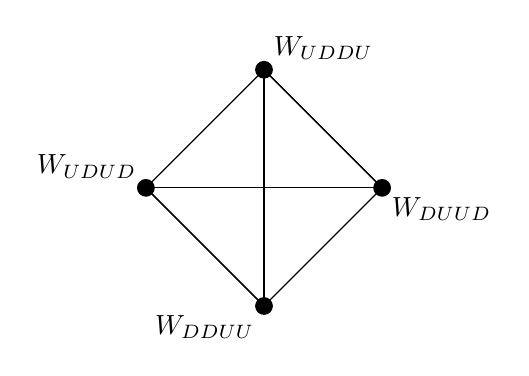
\begin{tikzpicture}[scale=1.5]
    % Define coordinates for the vertices
    \coordinate (A) at (0,0);
    \coordinate (B) at (1,1);
    \coordinate (C) at (2,0);
    \coordinate (D) at (1,-1);
    
    % Draw the vertices
    \filldraw[black] (A) circle (2pt) node[above left] {$W_{UDUD}$};
    \filldraw[black] (B) circle (2pt) node[above right] {$W_{UDDU}$};
    \filldraw[black] (C) circle (2pt) node[below right] {$W_{DUUD}$};
    \filldraw[black] (D) circle (2pt) node[below left] {$W_{DDUU}$};
    
    % Draw the edges with arrows
    \draw[->] (A) -- (B);
    \draw[->] (B) -- (C);
    \draw[->] (C) -- (D);
    \draw[->] (D) -- (A);
    \draw[->] (A) -- (C);
    \draw[->] (B) -- (D);
    \draw[->] (A) -- (D);
    \draw[->] (B) -- (C);
\end{tikzpicture}

\end{document}